\documentclass[10pt,a4paper,twoside]{article}
\usepackage[english]{babel}
%laad de pakketten nodig om wiskunde weer te geven :
\usepackage{amsmath,amssymb,amsfonts,textcomp}
%laad de pakketten voor figuren :
\usepackage{graphicx}
\usepackage{float,flafter}
\usepackage{hyperref}
\usepackage{inputenc}
\usepackage{minted}
\usepackage{subcaption}

\setlength\paperwidth{20.999cm}\setlength\paperheight{29.699cm}\setlength\voffset{-1in}\setlength\hoffset{-1in}\setlength\topmargin{1.499cm}\setlength\headheight{12pt}\setlength\headsep{0cm}\setlength\footskip{1.131cm}\setlength\textheight{25cm}\setlength\oddsidemargin{2.499cm}\setlength\textwidth{15.999cm}

\newcommand{\sweepsize}{0.26}

\begin{document}
\begin{center}
\hrule

\vspace{.4cm}
{\bf {\Huge Computer Vision} \\ {\huge Lab Assigment Report} \\ {\Large Condensation Tracker}}
\vspace{.2cm}
\end{center}
{\bf Tuan Mate Nguyen}  (tunguyen@student.ethz.ch)
\hrule


\section{Implementation}
\subsection{Color histogram}
For the histogram only pixels in the bounding box of the ROI are considered. This sub-array is then flattened as
required by np.histogramdd(), which is a function for creating multidimensional
histograms. As there are 3 color channels and $hist\_bin$ number of bins for each
color dimension, the resulting histogram will have a size of $hist\_bin^3$.

\begin{minted}[mathescape,
    linenos,
    numbersep=5pt,
    gobble=2,
    frame=lines,
    framesep=2mm,
    firstnumber=4]{csharp}
    roi = frame[ymin:ymax, xmin:xmax]
    flat_roi = roi.reshape(-1, 3)
    hist, _ = np.histogramdd(flat_roi, hist_bin, [[0, 255]]*3, density=False)
\end{minted}

The density parameter is set to false in order to obtain the number of samples in
each bin. Then the bins are explicitly normalized by dividing the total number of
samples.

\subsection{$A$ matrix}
In case of no motion the state vector consist of only two elements,
corresponding to the $x$ and $y$ coordinates of the object. Since the prediction
model assumes no motion, the coordinates remain the same after applying the
deterministic part of the system transition function. Thus, the $A$ matrix will
just be the identity matrix

\[ A_{no motion} =
\begin{bmatrix}
    1 & 0 \\
    0 & 1 
\end{bmatrix}
\]

As for the constant velocity model, the state vector has 4 elements, the two
spatial coordinates and the velocities in the $x$ and $y$
directions. For the new coordinates - ignoring dimensions - the deterministic
transition function can be written as

\[ x_t = x_{t-1} + v_{x_{t-1}} \]
\[ y_t = y_{t-1} + v_{y_{t-1}} \].

The velocities remain constant so in the bottom block the diagonal elements will
be 1 and everything else 0.

\[ A_{const. velocity} =
\begin{bmatrix}
    1 & 0 & 1 & 0 \\
    0 & 1 & 0 & 1 \\ 
    0 & 0 & 1 & 0 \\ 
    0 & 0 & 0 & 1 \\ 
\end{bmatrix}
\]

\subsection{Propagation}

The system then can be propagated by computing
\[
s_t^{(n)} = A{s^{'}}_{t-1}^{(n)} + w_{t-1}
\]
for every particle. Here $w_{t-1}^{(n)}$ is of shape (2,2) for the no motion
model (coordinate noise only) and (4,2) for the constant velocity model (both
coordinate and velocity perturbations). Its values are obtained by sampling from
a normal distribution with 0 mean and $\sigma_{pos}$ and $\sigma_{vel}$
standard deviation for the coordinates and velocities, respectively.

This operation could potentially result in particles located outside of the
frame. The chosen method to handle this is to clamp the updated coordinates so
that they remain inside the frame.

\begin{minted}[mathescape,
    linenos,
    numbersep=5pt,
    gobble=2,
    frame=lines,
    framesep=2mm,
    firstnumber=21]{csharp}
    xs = new_particles[:,0] < 0
    ys = new_particles[:,1] < 0
    new_particles[xs, 0] = 0
    new_particles[ys, 1] = 0
    
    xs = new_particles[:,0] >= frame_width
    ys = new_particles[:,1] >= frame_height
    new_particles[xs, 0] = frame_width-1
    new_particles[ys, 1] = frame_height-1
\end{minted}


\subsection{Observation}

In the observation step for each particle, first the bounding box needs to be
determined. The corner points can then be fed to the previously described color
histogram computing function. It is worth mentioning that in my implementation
objects on the image border will have a smaller bounding box than the original.
This could lead to slightly different color histogram as only a portion of the
object's colors are taken into account.  However, since the output doesn't
matter once the object leaves the frame, this is acceptable. Then the current
color histogram can be compared to the original one by taking their $\chi^2$
distance. The weight will be the Gaussian of this distance, parameterized by 0
mean and $\sigma_{observe}$ standard deviation. 

\begin{minted}[mathescape,
    linenos,
    numbersep=5pt,
    gobble=2,
    frame=lines,
    framesep=2mm,
    firstnumber=13]{csharp}
    # for every particle
    xmin = min(max(0, round(p[0]-half_w)), frame_width-1)
    ymin = min(max(0, round(p[1]-half_h)), frame_height-1)
    xmax = min(max(0, round(p[0]+half_w)), frame_width)
    ymax = min(max(0, round(p[1]+half_h)), frame_height)

    current_hist = color_histogram(xmin, ymin, xmax, ymax, frame, hist_bin)
    chi_dist = chi2_cost(hist, current_hist)
    weight = 1./(np.sqrt(2 * np.pi) * sigma_observe) * 
             np.exp(-1*(chi_dist * chi_dist) / (2 * sigma_observe * sigma_observe))
\end{minted}

Since the weights are used in a probabilistic context in the sampling step, we
need to normalize them so that their sum is 1.

\subsection{Estimation}

The mean state implementation is straight-forward, just taking a weighted sum of all particle states using their weights.
\begin{minted}[mathescape,
    linenos,
    numbersep=5pt,
    gobble=2,
    frame=lines,
    framesep=2mm,
    firstnumber=4]{csharp}
    mean_state = np.sum(particles * particles_w, axis=0)
\end{minted}

\subsection{Resampling}

For resampling first the particles and their current weights are paired so that
the resampled particles' weights are known.
\begin{minted}[mathescape,
    linenos,
    numbersep=5pt,
    gobble=2,
    frame=lines,
    framesep=2mm,
    firstnumber=4]{csharp}
    p = np.concatenate((particles, particles_w), axis=1)
\end{minted}
The sampling with replacement is convenient with numpy's random.Generator.choice() method, where the
chosen random number generator is the default one. The result is separated back into to particles
and their weights, and the weights are normalized (their sum is 1).
\begin{minted}[mathescape,
    linenos,
    numbersep=5pt,
    gobble=2,
    frame=lines,
    framesep=2mm,
    firstnumber=6]{csharp}
    # rng is a global variable: np.random.default_rng()
    p_new = rng.choice(p, size=particles.shape[0], replace=True, p=particles_w.reshape(-1), axis=0)
    n_dim = particles.shape[1]
    sampled_particles = p_new[:, :n_dim]
    sampled_weights = p_new[:, n_dim]
    sampled_weights = sampled_weights / np.sum(sampled_weights)
\end{minted}

\section{Experiments}

For the following coordinates instead of selecting the starting bounding boxes
manually every time, I hardcoded them to the following values to make comparison
between different paramters more accurate.
\begin{table}[h!]
\begin{center}
    \begin{tabular}{ c c c } 
     \hline
     Video & Top left & Bottom right\\
     \hline
     \hline
     1 & (128, 99)& (142, 111)\\ 
     \hline
     2 & (7, 70)&(20, 87)\\
     \hline
     3 & (24, 87)&(31, 95)\\
     \hline
    \end{tabular}
\end{center}
\end{table}    

\subsection{Video 1}

For the no motion model even the default values worked fairly well. Small
$\sigma_{position}$ version was a bit noisier. 

Number of particles was 100, 200, 300 resulting similar quality. In this case it
didn't really matter compared to 30 points, but in later videos using more
points proved to be more robust. In every case, the number of points were set to 300.

Different bin numbers (4, 16, 32) yielded similar results, at 64 the tracked trajectory became too noisy.

Updating the appearance model helped, after setting the $\alpha$ value higher
than $0.5-0.7$ results were more accurate. Without updating the center of the
hand was missed (mean was located slightly below, where the arm was similarly
dark as original hand).
%appearance model: 0.1 false track, 0.3 < 0.5~0.7~0.9~1.0 best so far
%with 0 it always stays bit below hand -> darker image originally; with update its more the center

The constant velocity model didn't work as well as the no motion model. This is
not surprising, as the motion was not constant but had sudden direction changes.
To handle these changes in velocity, $\sigma_{velocity}$ would need
to be big enough (comparable with initial velocity) so velocity could follow the
change but that would lead to sparser sampling, making the system less stable. A
solution could to use more points, but computing power is a limiting factor.

In general sudden movements are better modeled assuming no motion and just using
bigger standard deviation (because positions are independently generated for
every frame, but for the constant velocity model the previous velocity vector influences new coordinates).

\subsection{Video 2}

Using best model from previous case doesn't work: tracking is lost after occlusion

solutions:
don't update so much alpha=0.1 still doesn't work but almost, 0.0 works but gets confused at the end
as the object is occluded by at least 50\% for several frames, alpha could significantly reduce the performance
so lets fix alpha=0

Let's change system model!
Constant velocity model's effect:
More robust agains temporary occlusion: on average, as the constant velocity is
kept (if tuned well in the beginning), the position distribution will be shifted
by the constant velocity FOR EVERY FRAME. so eventhough the std.dev of position
noise is not big enough tracking is not lost
RESULT: pass occlusion


??? When does it work nicely?
Using previous settings with v=(3,0) and sigma vel. =  it works nicely


Effect of changing system noise:
smaller vel.noise will result in just bad motion, regardless of actual motion as not enough sample points to find target area
if larger vel.noise causes then initial difference from object could quickly increase and trackign would deviate significantly
(sigma=2,8)

Effect of changing measurement noise:
big noise asymptotically would mean that we sample from particles uniformly regardless of their resemblance to the object.
In a range it works as points close enough to the object will still have
relatively high weight. If too high, then only the perfect particle'd be kept but
their position is random, so probably tracking will be lost. (weights of totally
different and quite close particles will have the same order of magnitude.) as the choice again will be random.

measurement: determine velocity by measurement!
????too small pos noise: in case of no motion tracking is blocked by the occlusion. Sensible, we're confident that 




other:
tracking for different alpha values if pos noise is 0, vel noise is 0.5, v =3,0.2
 - 0.3 doesn't work, 0.2 works


\subsection{Video 3}
In this case the appearance doesn't need to be updated because there's a big
contrast between the ball and the background and there's no occlusion, thus
$\alpha$ was kept 0.

The no motion model works well as long as the position noise is comparable with
$v_x$ so there're sufficiently enough samples near the ball.
If the position system noise is too small the ball will quickly be outside the
sampled area (that is, the probability of points in its neighborhood being
sampled will be too small).
\begin{figure}[h]
    \centering
    \begin{subfigure}{\sweepsize\textwidth}
    \includegraphics[width=0.9\linewidth]{3/3_hb32_np300_mm0_am0.0_sp3_sv5_4.png} 
    \caption{$bandwidth=1.8$}
    \end{subfigure}
    \begin{subfigure}{\sweepsize\textwidth}
    \includegraphics[width=0.9\linewidth]{3/3_hb32_np300_mm0_am0.0_sp3_sv5_11.png} 
    \caption{$bandwidth=2.5$}
    \end{subfigure}
    \begin{subfigure}{\sweepsize\textwidth}
    \includegraphics[width=0.9\linewidth]{3/3_hb32_np300_mm0_am0.0_sp3_sv5_17.png} 
    \caption{$bandwidth=3.8$}
    \end{subfigure}
    \begin{subfigure}{\sweepsize\textwidth}
    \includegraphics[width=0.9\linewidth]{3/3_hb32_np300_mm0_am0.0_sp3_sv5_23.png} 
    \caption{$bandwidth=5$}
    \end{subfigure}
    \begin{subfigure}{\sweepsize\textwidth}
    \includegraphics[width=0.9\linewidth]{3/3_hb32_np300_mm0_am0.0_sp3_sv5_29.png} 
    \caption{$bandwidth=3.8$}
    \end{subfigure}
    \begin{subfigure}{\sweepsize\textwidth}
    \includegraphics[width=0.9\linewidth]{3/3_hb32_np300_mm0_am0.0_sp3_sv5_35.png} 
    \caption{$bandwidth=5$}
    \end{subfigure}
    \caption{$\sigma_{pos}=3$ is too small, sampled points can't keep up with
    the ball, position remains constant (until ball rolls back)}
\end{figure}

\begin{figure}[h]
    \centering
    \begin{subfigure}{\sweepsize\textwidth}
    \includegraphics[width=0.9\linewidth]{3/3_hb32_np300_mm0_am0.0_sp7_sv5_4.png} 
    \caption{$bandwidth=1.8$}
    \end{subfigure}
    \begin{subfigure}{\sweepsize\textwidth}
    \includegraphics[width=0.9\linewidth]{3/3_hb32_np300_mm0_am0.0_sp7_sv5_11.png} 
    \caption{$bandwidth=2.5$}
    \end{subfigure}
    \begin{subfigure}{\sweepsize\textwidth}
    \includegraphics[width=0.9\linewidth]{3/3_hb32_np300_mm0_am0.0_sp7_sv5_17.png} 
    \caption{$bandwidth=3.8$}
    \end{subfigure}
    \begin{subfigure}{\sweepsize\textwidth}
    \includegraphics[width=0.9\linewidth]{3/3_hb32_np300_mm0_am0.0_sp7_sv5_23.png} 
    \caption{$bandwidth=5$}
    \end{subfigure}
    \begin{subfigure}{\sweepsize\textwidth}
    \includegraphics[width=0.9\linewidth]{3/3_hb32_np300_mm0_am0.0_sp7_sv5_29.png} 
    \caption{$bandwidth=3.8$}
    \end{subfigure}
    \begin{subfigure}{\sweepsize\textwidth}
    \includegraphics[width=0.9\linewidth]{3/3_hb32_np300_mm0_am0.0_sp7_sv5_35.png} 
    \caption{$bandwidth=5$}
    \end{subfigure}
    \caption{$\sigma_{pos}=7$, roughly same as $v_x$ (ignoring the dimensionality)}

\end{figure}

Constant velocity model approximate well the ball's motion until it hits the
wall. Then it's lost of course as velocity in the $x$ coordinate will be the
opposite, while the model assumes consant motion.
To handle this the noise needs to be roughly twice as big as the initial
velocity. However, it's not robuse because in this case the velocity vector easily deviates from the
ball. As mentioned above, more sampling points could help with this, were computing power not a limiting factor.
%alpha=0, sigma pos=2, sigma vel5, vel=5,0 is nice!

\begin{figure}[h]
    \centering
    \begin{subfigure}{\sweepsize\textwidth}
    \includegraphics[width=0.9\linewidth]{3/3_hb32_np300_mm1_am0.0_sp2_sv2_4.png} 
    \caption{$bandwidth=1.8$}
    \end{subfigure}
    \begin{subfigure}{\sweepsize\textwidth}
    \includegraphics[width=0.9\linewidth]{3/3_hb32_np300_mm1_am0.0_sp2_sv2_11.png} 
    \caption{$bandwidth=2.5$}
    \end{subfigure}
    \begin{subfigure}{\sweepsize\textwidth}
    \includegraphics[width=0.9\linewidth]{3/3_hb32_np300_mm1_am0.0_sp2_sv2_17.png} 
    \caption{$bandwidth=3.8$}
    \end{subfigure}
    \begin{subfigure}{\sweepsize\textwidth}
    \includegraphics[width=0.9\linewidth]{3/3_hb32_np300_mm1_am0.0_sp2_sv2_23.png} 
    \caption{$bandwidth=5$}
    \end{subfigure}
    \begin{subfigure}{\sweepsize\textwidth}
    \includegraphics[width=0.9\linewidth]{3/3_hb32_np300_mm1_am0.0_sp2_sv2_29.png} 
    \caption{$bandwidth=3.8$}
    \end{subfigure}
    \begin{subfigure}{\sweepsize\textwidth}
    \includegraphics[width=0.9\linewidth]{3/3_hb32_np300_mm1_am0.0_sp2_sv2_35.png} 
    \caption{$bandwidth=5$}
    \end{subfigure}
    \caption{$\sigma_{pos}=2$, $\sigma_{velocity}=2$, smaller than $v_x=7$ (ignoring the dimensionality). After sharp change of direction tracking is lost.}

\end{figure}

\section{Further questions}
\subsection{Number of particles}

It's always good if the number of sampled particles is as high as possible
(depending on available computing resources). This is especially important if
the velocity of the obejct can suddenly change either in its direction or in its
magnitude.

\subsection{Number of bins}

Fewer number of bins make the observation less sensitive to the color histogram.
This could work if there's a high contrast between the object (foreground) and
background. The performance will degrade, however, if these have similar colors.

More bins could allow for better distinction of histograms and more accurate tracking. This requires a
higher quality footage (it's more sensitive to color noise) and enough sampling
points that there's always a high probabilty that the ROI will be sampled. Also,
it's better if the tracked area is bigger so its histogram is more reliable.

\subsection{Appearance model update}
Updated model is better when the appearance of the object being tracked changes
in time (for example, illumination changes). In this case performance is more
robust if tracking is always fairly accurate.

The disadvantage becomes clear when it's not always accurate enough and the object is
lost. For instance, this could be the case when the object becomes fully
occluded in a frame and
none of the propagated states reflect the actual state correctly. Then
- especially if using a high alpha value - the system could "forget" how the object looked
like and could keep tracking based on the wrong mean state since it will sample
some particales regardless of the fact that none of them is correct.


% Python code
%\begin{minted}[mathescape,
%    linenos,
%    numbersep=5pt,
%    gobble=2,
%    frame=lines,
%    framesep=2mm,
%    firstnumber=26]{csharp}
%\end{minted}

% Image
%\begin{figure}[H]
%    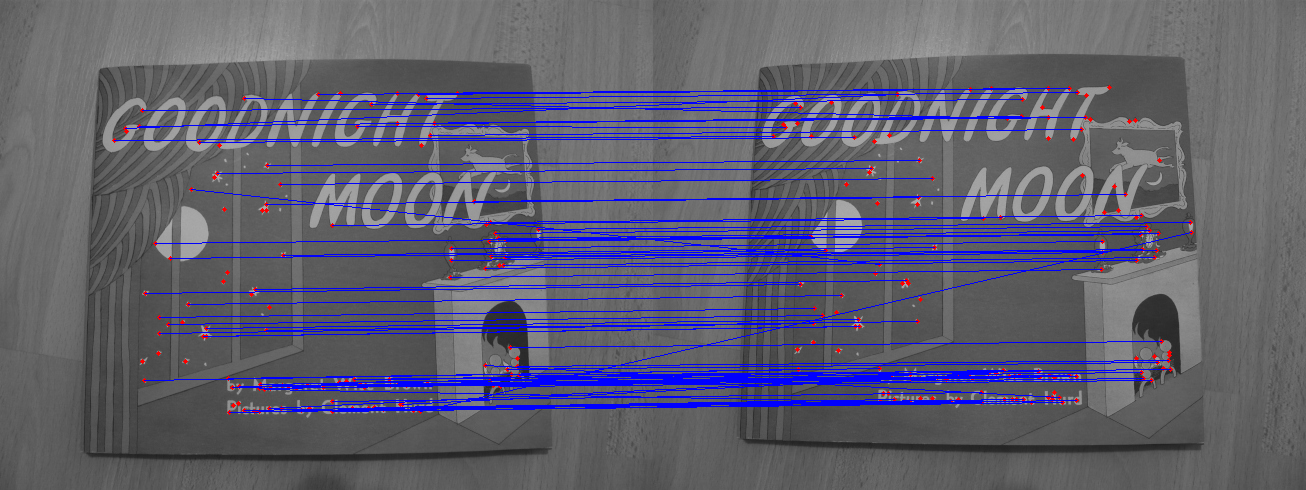
\includegraphics[width=\textwidth]{match_mutual.png}
%    \centering
%    \caption{Matching keypoints for mutual nearest neighbor matching}
%    \label{match_mutual}
%\end{figure}

\end{document}
